% Chapter Template

\chapter{In Graph Index Structure: Experiments \& Analysis} % Main chapter title

\label{Chapter 5} % Change X to a consecutive number; for referencing this chapter elsewhere, use \ref{ChapterX}

In this chapter we start by describing how to modify existing gremlin queries to use the index structure that was created in the previous chapters. We go in a sequential manner describing small modifications \& doing the associated error analysis - slowly building towards the final model that we have in our code repository currently. This will help user appreciate why a particular modification was needed and also help him/her reason about any further optimization that can be brought into the query.

\section{Modifying the Gremlin}

Let us take the example of query from chapter 2 (the one given as a sample).

\begin{lstlisting}
g.V().hasLabel("post", "comment")
  .has("po_creationDate", P.lt(dateVar))
  .group()
  .by{ it.value("po_creationDate").getYear()+1900 }
  .by(group().by(T.label).by(group().by{
    int len = it.value("length");
    if (len < 40) {
        return "short";
    } else if (len < 80) {
        return "one liner";
    } else if (len < 160) {
        return "tweet";
    } else {
        return "long";
    }}));
\end{lstlisting}
To be able to use our in graph index structure in processing of this query the most obvious way is that of retrieving the vertices based on the index structure first and then passing them to the graph traversal for further processing down the line. Let us assume that we have a function of `searchRange' already at our disposal that using our index structure can retrieve all the vertices based on the attribute conditions. Then using this our modified query will look something like below:

\begin{lstlisting}
vertices = (new IndexRangeQuery())
              .searchRange(g, 
                     dateFormat.parse(initDateVar),
                     dateFormat.parse(dateVar),
                     indexName);

g.V(vertices).hasLabel("post","comment")
  .group()
  .by{ it.value("po_creationDate").getYear()+1900 }
  .by(group().by(T.label).by(group().by{
    int len = it.value("length");
    if (len < 40) {
        return "short";
    } else if (len < 80) {
        return "one liner";
    } else if (len < 160) {
        return "tweet";
    } else {
        return "long";
    }}));
\end{lstlisting}
The `searchRange' function can be written in Java, using the gremlin-java support, that enables us to write a simplistic B+Tree traversal code in Java to traverse the above created index. Reader can look at the code repository to get a deeper understanding of how this was exactly done. The observed performance comparison for this kind of query vs the one using the external indexing application (elastic search in this case) is shown below:
$\:$\\
\begin{figure}[H]
\centering
\begin{minipage}{0.5\textwidth}
  \centering
  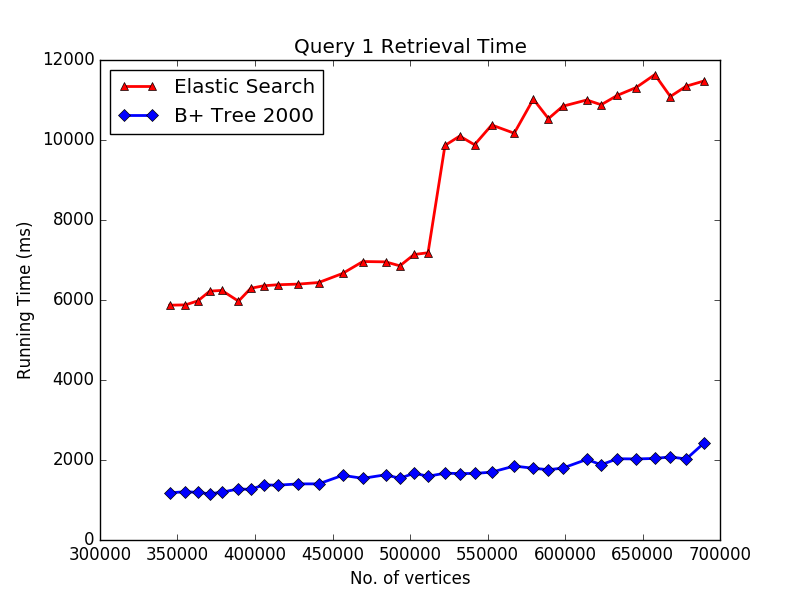
\includegraphics[width=.8\linewidth]{Figures/figure_2}
  \captionof{figure}{Vertex Retrieval Time}
  \label{fig:test1}
\end{minipage}%
\begin{minipage}{.5\textwidth}
  \centering
  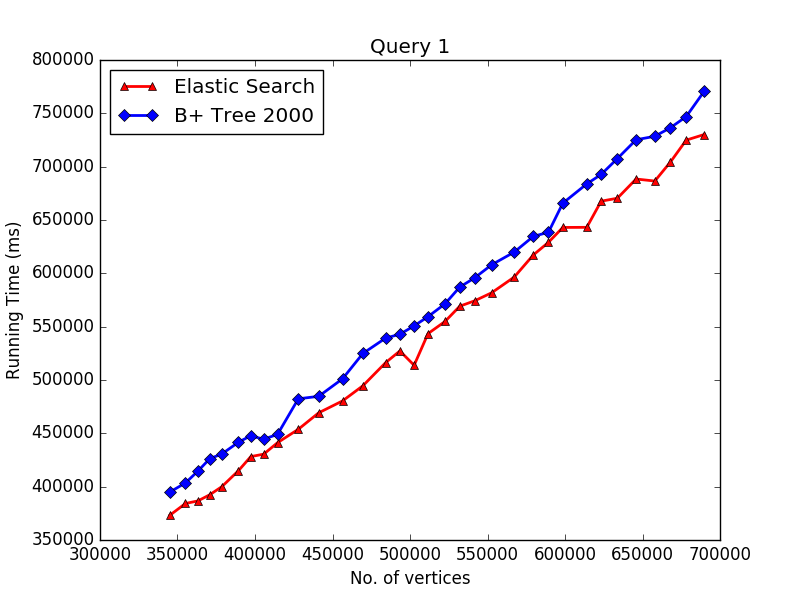
\includegraphics[width=.8\linewidth]{Figures/figure_1}
  \captionof{figure}{Query Running Time}
  \label{fig:test2}
\end{minipage}
\end{figure}
$\:$\\
From the graph we can see that though the in graph index structure out performs the elastic search index in terms of just the data retrieval (the primary task of the index), the in graph data index has somehow caused the overall query to slow down. 

\subsection{Hyperparameter: Fan-out factor}
The in graph indexed used to produce the above results is a B+ Tree with a fan out factor of 2000 (i.e. maximum no. of children of a node is 2000). This is a hyper-parameter that can be searched over to get the most optimal value. For our experiments we did not perform any hyper parameter search but instead chose an intuitive value after checking the query timings with a few values of the fan out factor. 

\section{Error analysis and optimizations}
In the above section we observed a that the query utilizing the in graph index data structure was slower than the query utilizing the elastic search index. A prominent reason behind this could be that the in the query using the in graph index data structure, there is an explicit separation of the data retrieval step and data processing step. While on the other hand the query utilizing the elastic search index might derive benefits from pipelining of the two parts of the query. (Note: Pipelining, here, refers to the general definition of pipelining popular in the DBMS community). In order to confirm this hypothesis, a simple experiment would be to separate the query utilizing the elastic search index into two parts and obtain the query timings. Shown below is the query timing graph for such a case. 

\begin{figure}[H]
\centering
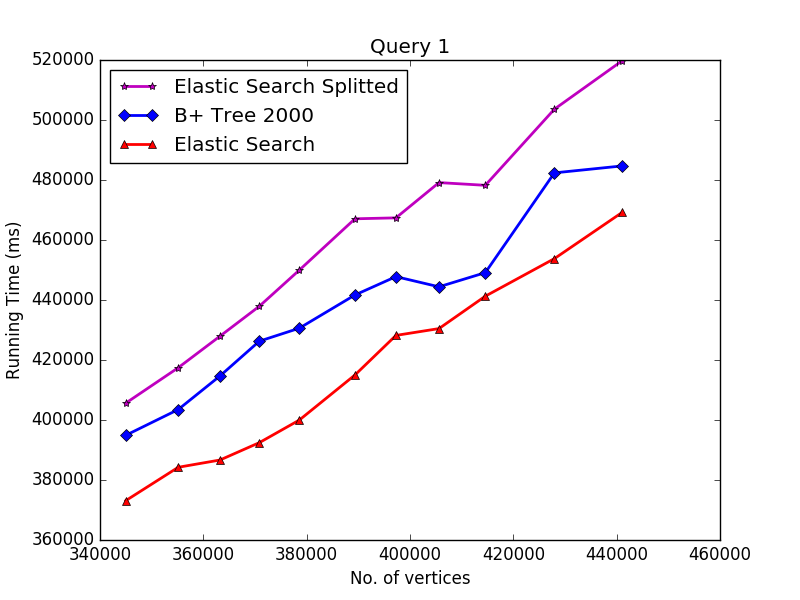
\includegraphics[width=.8\linewidth]{Figures/figure_1-100}
\captionof{figure}{Query Running Time}
\label{fig:test1}
\end{figure}
$\:$\\
While we now have some idea on what might be going wrong, how this can be rectified is still to be resolved. As an attempt to resolve this we try to combine the two parts of the query utilizing the in graph index structure into one. This can be done by traversing the index to retrieve information in a single gremlin query rather than in Java-like code and then calling the data processing steps on this traversal.  We used .repeat() and .until() steps to traverse over our in graph index data structure. The traversal that we came up with to traverse through the B+ Tree in a single gremlin query is shown below:
\\
\begin{lstlisting}
g.V().has("index_id", -1).out().has("name",indexName)           //index root
  .repeat(
    __.outE("INDEX_EDGE")
      .not(__.has("min", P.gte(dateVar)))
      .not(__.has("max", P.lte(initDateVar)))
      .inV()
  )
  .until(__.outE("INDEX_EDGE").count().is(0))
  .outE("INDEX_DATA_EDGE")
  .has("val", P.gte(initDateVar)).has("val", P.lte(dateVar)).inV()
\end{lstlisting}
$\:$\\
Combining this with the data processing step from the sample query we have been using, we get a combined query as shown below:
\\
\begin{lstlisting}
g.V().has("index_id", -1).out().has("name",indexName)
  .repeat(
    __.outE("INDEX_EDGE")
      .not(__.has("min", P.gte(dateVar)))
      .not(__.has("max", P.lte(initDateVar)))
      .inV()
  )
  .until(__.outE("INDEX_EDGE").count().is(0))
  .outE("INDEX_DATA_EDGE")
  .has("val", P.gte(initDateVar)).has("val", P.lte(dateVar)).inV()
  .group()
  .by{ it.value("po_creationDate").getYear()+1900 }
  .by(group().by(T.label).by(group().by{
    int len = it.value("length");
    if (len < 40) {
        return "short";
    } else if (len < 80) {
        return "one liner";
    } else if (len < 160) {
        return "tweet";
    } else {
        return "long";
    }}));
\end{lstlisting}
$\:$\\
The comparison of this query with the one utilizing elastic search is shown below. The elastic search index is still out performing ours in terms in the full query time. 

\begin{figure}[H]
\centering
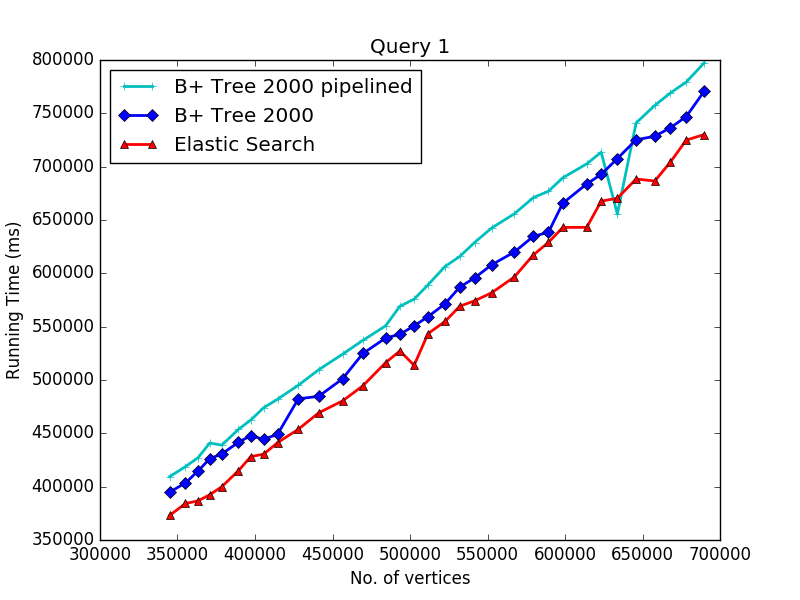
\includegraphics[width=.8\linewidth]{Figures/figure_1-200}
\captionof{figure}{Query Running Time}
\label{fig:test1}
\end{figure}
$\:$\\
Clearly we have not been able to come up with the optimal index traversal gremlin query. We experiment with a few things like if the order of the data retrieved is affecting the overall processing time but have not received any convincing results yet. One prime thing we came across was the bulk optimizations that are internal to JanusGraph. Interestingly putting an explicit barrier step after data retrieval does the greatest improvement to our timings.
\begin{figure}[H]
\centering
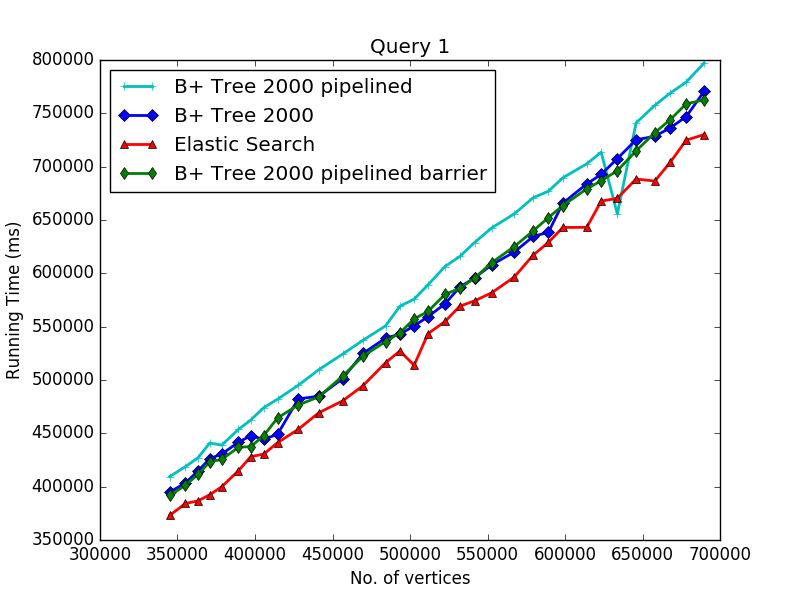
\includegraphics[width=.8\linewidth]{Figures/figure_1-300}
\captionof{figure}{Query Running Time}
\label{fig:test1}
\end{figure}
$\:$\\
In order to obtain greater insights on what was going wrong we started looking at other queries in the workload and surprisingly there were quite a few of them where the queries utilizing our index executed faster than the ones utilizing the elastic search index. This has been shown below:

\begin{figure}[H]
\centering
\begin{minipage}{0.33\textwidth}
  \centering
  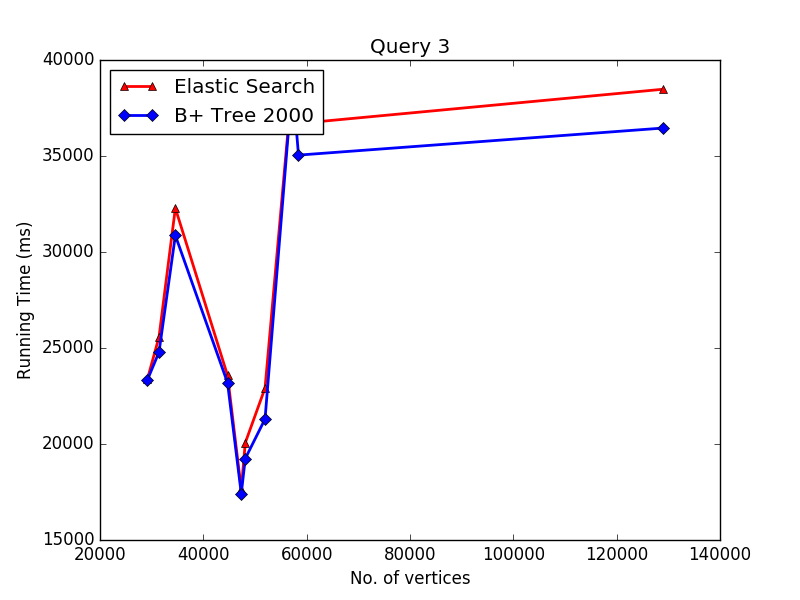
\includegraphics[width=1\linewidth]{Figures/figure_3}
  \captionof{figure}{}
  \label{fig:test1}
\end{minipage}%
\begin{minipage}{.33\textwidth}
  \centering
  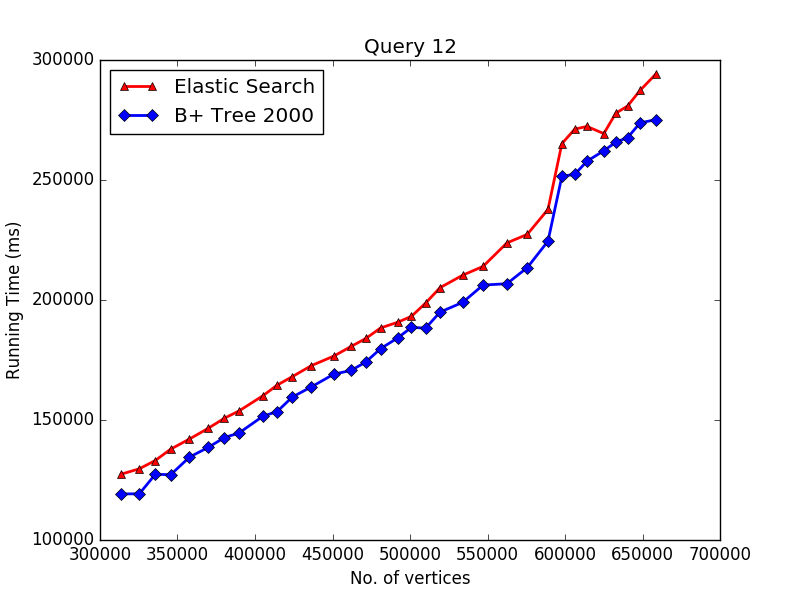
\includegraphics[width=1\linewidth]{Figures/figure_12}
  \captionof{figure}{}
  \label{fig:test2}
\end{minipage}
\begin{minipage}{.33\textwidth}
  \centering
  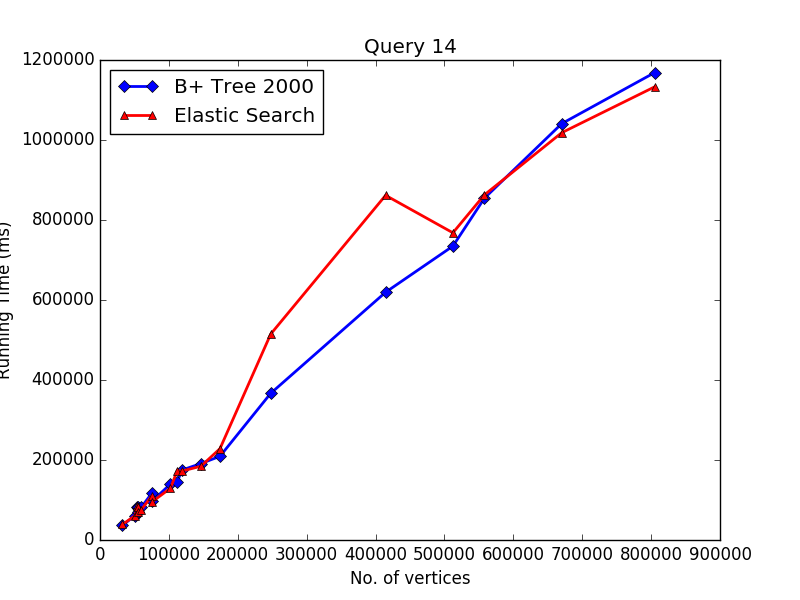
\includegraphics[width=1\linewidth]{Figures/figure_14-1}
  \captionof{figure}{}
  \label{fig:test2}
\end{minipage}
\end{figure}
$\:$\\
Why the performance in query 1 degrades is something that remains to the ascertained yet. How can we further improve the performance and make this much more faster than elastic search would be another interesting thing to explore and find out.

% \subsection{The Queries module}
% The Queries are in the codebase all inherit from the \textit{Query} class. This enforces the Query classes to have a function runQuery() that returns an object of \textit{QueryResult}. The \textit{QueryResult} object allows storage of various parameters that are useful in query runtime analysis. These are
% \begin{itemize}
% \item Count of vertices returned
% \item Time to run query
% \item Time to traverse index
% \item The result returned
% \end{itemize}




\section{Results}

\paragraph{The result sheet}
$\:$\\
The aforementioned Google Sheet \cite{runtime} contains all the experimental results we have obtained. The sheets \textit{[Final] Query Running Time} and \textit{[Final] Vertex Retrieval Time} contain our final query timings when we ran them on Aryabhata on the 1GB dataset. We have the timings for queries 1, 3, 10, 12 and 14. These are the queries that used our B+ Tree index on \textit{po\_creationDate} property.

\section{Brief description of the code repository}

\paragraph{PerformanceTester}
$\:$\\
\textit{PerformanceTester} is a class created to aid the running of queries to get reliable experimental data of run times. This class runs the queries in the Queries folder. These queries are expected to inherit from the \textit{Query} class. The \textit{PerformanceTester} takes the class name of query to run, the parameter file index in \textit{substitution\_parameter} folder, the number of lines to skip in the parameter file and the \textit{conf} file to use to make connection to the JanusGraph DB.
\\\\
Running the \textit{PerformanceTester} runs the specified query using the specified parameter file. It generates a .txt file that has various metrics like the average, median and standard deviation of the query run times and the index traversal times. This .txt file is generated in a \textit{query\_results} folder.


\paragraph{Using the Performance Tester class}
$\:$\\
Create the jar of the java module. The usage for running the jar is
\\\\
\textit{java -cp Utilities-1.0-SNAPSHOT-jar-with-dependencies.jar main.PerformanceTester\\<queryClassName(only the endclassname)> <param\_number> <skiplines> [<confFile>]}
\\\\
Example:
\\
\textit{java -cp Utilities-1.0-SNAPSHOT-jar-with-dependencies.jar main.PerformanceTester BPIndexQuery1\_1 1 1 local}
\\\\
The \textit{query\_results}, \textit{substitution\_parameter} and \textit{conf} folder will need to be present along with the jar when it is run. Sample of these can be obtained from our git repository \cite{repo}.
\\\\
The times we obtained by running queries can be accessed at result spreadsheet\cite{runtime}



